\documentclass[11pt]{report}
\usepackage{graphicx}
\usepackage[text={16cm,24cm},centering]{geometry}
\usepackage[%  
colorlinks=false,
pdfborder={0 0 0},
]{hyperref}
\usepackage{xcolor}
\usepackage{enumerate}% Roman numerals
\usepackage{paracol} % For parallel colums
\usepackage{subcaption}
\usepackage{harpoon} % For vector notation
\usepackage{amsmath} % For matrices. And vectors?
\usepackage{mathtools} % For vector notation again
\usepackage{bm} % Also for vector notation again
\usepackage[title]{appendix}

\renewcommand{\thesection}{\arabic{section}}

\renewcommand\bibname{References}

\renewcommand{\vec}[1]{\mathbf{#1}} % For vector notation

\setcounter{tocdepth}{4}
\setcounter{secnumdepth}{4}

\begin{document}
		%% This document creates the title page for the report


%% Document settings
%{

\newcommand{\HRule}{\centering{\rule{.9\linewidth}{.6pt}}} % New command to make the lines in the title page

\newcommand{\decoRule}{\rule{.8\textwidth}{.4pt}} % New command for a rule to be used under figures

%}

\begin{titlepage}
   
      %% Title Images
   	  \hspace{-2cm}
   	  
\includegraphics[
   	  width=0.30\textwidth,
   	  height=0.3\textheight
   	  ]{resources/wits-stacked.jpg}
   	  \hspace{0.50\textwidth}
   	  
\includegraphics[
   	  width=0.5\textwidth
   	  ]{resources/eie-full.png}
     
 \begin{center}
 	
 	
   	    \vspace*{\fill}
   	 	%% Title
      	\textsc{
      		\LARGE
      		ELEN4011: Design II
      	}
      
      	\HRule \\[0.4cm] % Horizontal line
      
      	\textsc{
      		\LARGE
      	Design of a robust codec for a fading channel.}
      
      	\HRule \\[1.5cm] % Another Horizontal line
      	
      	%% Author
      	
      	\hspace{0.60cm} Author \hspace{4.1cm} Supervisor\\
      	\hspace{0.45cm}\textsc{Elias Sepuru - 1427726} \hspace{1cm}\textsc{Prof. Fambirai Takawira}
      	
      	%% Thanks
      	{
      		\vspace{1cm}
      		School of Electrical and Information Engineering,
      		University of the Witwatersrand, Johannesburg 2050, South Africa
      		\\
        }
    	
    	%% Date
    	\vspace*{1cm}	
    	{25 October 2019}
    	
      	\vspace*{\fill}
    
 
   \end{center}
\end{titlepage}
\begin{abstract}
This paper presents the design of a robust codec for fading channel. The codec use BCH(127,64) for channel encoding, 16-QAM for modulation and a $4\times2$ Spatial Multiplexing MIMO antenna configuration. At the receiver of the MIMO architecture a MMSE receiver is used to equalise and sum the received distorted signals. The results show that modulation schemes greatly affect BER performance, they also show that more antennas improve diversity. Overall the codec achieved a spectral efficiency of 2.00 bits/Hz which meets the design requirements.  
\end{abstract}

\tableofcontents

\newpage

\section{Introduction}
\label{sec:intro}
The aim of modern and next-generation wireless communication systems is to provide communication services with high data rates and low probability of error, this also helps in catering for numerous requests from various applications and devices \cite{36,14,49}. The reliability of such communication systems is often hindered by strong shadowing, intersymbol interference (ISI) and attenuation due to the destructive addition of multipaths propagation in the transmission channel \cite{36,32}. Such a channel is often accurately modeled using a Rayleigh model known as the Rayleigh Fading Channel (RFC) \cite{32}. To combat the effect of fading and scattering due to RFC, several methods have been proposed. Methods such as Selection Diversity, Equal Gain Combining and Maximal Ratio Combining were proposed. However the methods proved to be inefficient and ineffective in dealing with the requirement of high data rates as per modern communication needs \cite{B8}. This lead to the development of Multiple-Input Multiple-Output (MIMO) systems. MIMO leverages off the multipath characteristic of the Rayleigh Fading Channel. It transmits data over the multiple paths, therefore increasing the amount of information the communication system carries \cite{50}. MIMO uses multiple transmit and receive antennas to significantly increase the data throughput and link range without additional bandwidth or transmit power \cite{B6}. However MIMO cannot 
achieve all this without robust Forward Error Correction (FEC) and modem schemes. 
\\
\\
This paper presents the design of a robust codec for a fading channel. The codec is to operate at a rate of at least 2 bits/Hz over a Raleigh Fading Channel. The design of the codec focuses mainly on FEC, modulation and MIMO. The codec input data input is expected to be at 10 Mbps. The design assumes that the data stream has already been converted from analog to digital, hence source encoding is neglected. Encryption is also left out as it does not affect the Bit Error Rate (BER) and spectral efficiency. The design also assumes that the channel coefficients of the Raleigh Fading Channel are known, hence there is no need for channel estimation. The below sections present the mathematical description of the designed codec together with testing, results and analysis. All simulations and computations are carried out in MATLAB.

\section{Design Overview}
\label{sec:design}
A typical digital communication system constitutes of three main components, those components being the transmitter, the channel and the receiver. Figure \ref{fig:sys} illustrates a typical communication system consisting of MIMO architecture. 
\\
\begin{figure}[h]
	\centering
	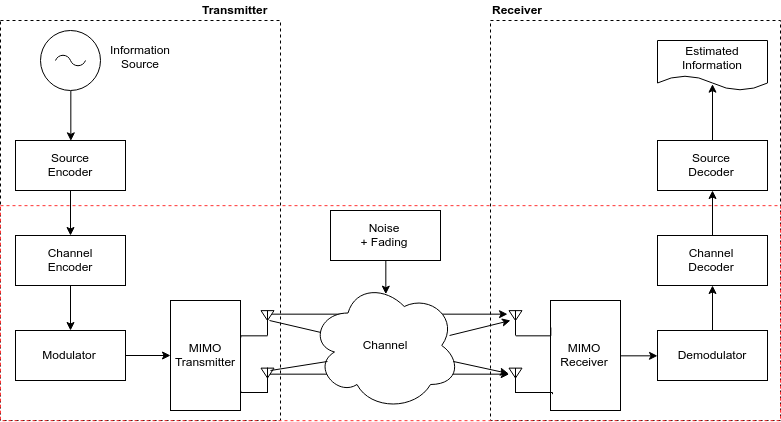
\includegraphics[width=\textwidth]{resources/systemDiagram.png}
	\caption{System block diagram of a typical communication system with MIMO architecture}
	\label{fig:sys}
\end{figure}{}
\\
From figure \ref{fig:sys}, it can be seen that the receiver mirrors the transmitter in most of the sub-components. 

\subsection{The Transmitter}
\label{sub:trans}

On the transmitter side, the source encoder takes in a raw message signal and converts it into a sequence of bits. This is done to compress the raw message data and to remove redundancy. The end result of source encoding is digital information bits with lesser bandwidth and just enough information to reconstruct the original message \cite{B10}. After source encoding, the information bits are sent to the channel encoder. The channel encoder uses FEC codes to add redundancy to the information bits. This is done to facilitate error detection and correction on the receiver side after channel transmission. The next step is modulation, the modulator takes in the coded bits from the channel encoder and maps them to a signal to be transmitted over the channel. This is done to conserve power and bandwidth. The MIMO transmitter takes in the symbols and transmits them over the channel using its multiple antennas. The MIMO transmitter uses multiple antennas to boost bandwidth and to improve signal range as mentioned earlier.

\subsection{The Channel}
The steps mentioned in section \ref{sub:trans} are taken so as to  prepare the original message to prevail in the channel and so that it is sent as efficiently as possible. The channel can be any medium, wireless or physical, into which the transmitted signal propagates. The channel distorts and adds noise to the transmitted signal, and in some instances interference occurs \cite{B10}. 

\subsection{The Receiver}
The mirrored side of of the transmitter, which is the receiver, performs the opposite of all the steps mentioned in section \ref{sub:trans} respectively. This done in order to recover the original sent message to the highest accuracy possible. 
\\
\\
This paper only focuses on the part of the communication system highlighted in red on figure \ref{fig:sys}.

\section{Channel Encoding}
\label{sec:encoding}
As mentioned earlier, transmitting data over a noisy channel often leads to the information being corrupted. To minimise the occurrence of errors during transmission the information has to somehow be protected. This protection is achieved through either the use of FEC codes or Automatic Repeat Requests (ARQ). ARQ requires retransmission of bits if they are in error. This leads to delays in communication, wasteful retransmissions that require additional power and bandwidth and also interference with other users \cite{B11}. All these make ARQ not suitable for real-time applications especially in interactive media applications \cite{51}. FEC on the other hand uses error correcting codes to correct errors that occur during transmission. It does this by adding redundant bits on the information bits, this helps to detect and correct errors as mentioned earlier. For this design FEC is chosen due to the fact that it offers improved BER, higher throughput and minimal delays compared to its counterpart \cite{51,52}.
\\
\\
FEC codes are split up into two categories: Convolutional Codes and Linear Block Codes. Error correcting capability and/or performance of an FEC coding scheme is measured by its code rate $r$. The code rate represented by equation \ref{eq:1} below.

\begin{equation}
r = \frac{k}{n}
\label{eq:1}
\end{equation}{}
\\
The code rate presents the proportion of the data stream that is useful to the one that has redundancy, represented by $k$ and $n$ respectively in equation \ref{eq:1}.

\subsection{Convolutional Codes}
\label{sub:conv}
Convolutional Codes are mostly used in applications that require real time error correction. They are generated by combining the input data stream bits in a series manner. The input bits are stored in a fixed length shift register and are combined with the use of modulo-2 adders \cite{53}. The output of the convolutional encoder at any point is a combination of the previous bits in the shift register.
\\
\\
One type of a Convolutional Codes are Turbo codes. Turbo codes are known to perform extremely well compared to any other FEC code. They achieve within a fraction of a dB of the Shannon Capacity in certain channels \cite{B11}. The major disadvantage of Convolutional Codes is their complexity. The complexity curve steepens even further when trying to decode them \cite{B11}. The simplest decoder which is the Viterbi also increase in complexity and it gets much difficult to implement for large codewords
\cite{54}.

\subsection{Linear Block Codes}
In Linear Block Codes, the resultant codeword is formed as a linear combination of two codewords. The two codewords are the original message bits having size $k$ and the parity bits of size $n-k$, where $n$ is the size of the resulting codeword.
\\
\\
There exist three main types of of Linear Block Codes used in coding theory: Bose Chaudhuri Hochquenghem (BCH), Reed Solomon (RS) and Low Density Parity Check (LDPC) codes. LDPC codes are regarded to be in the same league as Turbo codes with regards to performance. However, like Turbo codes they have major draw backs. LDPC codes require large sums of computation power, have low flexibility and have high encoding complexities \cite{59,56}.  RS codes, derived from BCH codes, are well known for their suitability when it comes to correcting burst errors. Compared with BCH, they were found to perform poorly in RFCs \cite{10,57}. Due to arguments raised in section \ref{sub:conv} and in this section BCH codes are chosen as the suitable candidate for this design.
\\
\\
BCH codes form a class of cyclic codes constructed using the principles of the Galois Finite Fields. Unlike RS codes, they are able to correct multiple random errors and unlike LDPC and Turbo codes, they are relatively easier to implement and decoding is also simple \cite{20,57}. Other great advantages of this coding scheme is its flexibility of choosing the number of errors correctable by the code and its great error correcting capabilities \cite{57,58,22}.

\subsubsection{BCH Encoder and Decoder}
BCH$(n,k)$ codes are a generalisation of Hamming Code. Unlike Hamming code, BCH$(n,k)$ posses the ability to correct multiple errors. They are described mathematically as follows:

\begin{center}
\begin{minipage}[h!]{0.85\textwidth}
  	
  	
  	{\it For any positive integers $m\ge3$ and $ t < 2^{m-1} $ there exists a BCH(n,k) code with the following characteristics:}
  	
  	\begin{equation}
  	\label{eq:block}
  	 \mbox{Block length: \hspace{1cm}} n = 2^{m-1}  	
  	\end{equation}
  	\begin{equation}
  	\label{eq:parity}
  	\mbox{Parity check bits: \hspace{1cm}} n -k \le mt 	
  	\end{equation}
  		\begin{equation}
  	\label{eq:dmin}
  	\mbox{Minimun distance: \hspace{1cm}} d_{min} \ge 2t + 1	
  	\end{equation}

\end{minipage}
\end{center}

A BCH$(n,k)$ code described by equations \ref{eq:block}$-$\ref{eq:dmin} is described as a $t$-error correcting BCH.
\\
\\
To encode, BCH codes uses a generator polynomial $g(x)$ defined in the Galois Field GF($2^m$). The polynomial is the lowest degree polynomial over GF(2) which has $\alpha, \alpha^2,...,\alpha^{2t}$ as its roots. If $\Phi(x)_i$ is a minimal polynomial of $\alpha_i$, then $g(x)$ is given by equation \ref{eq:gx} below,

\begin{equation}
\label{eq:gx}
	g(x) = LCM(\Phi(x)_1,\Phi(x)_3,...,\Phi(x)_{2t-1})
\end{equation}
\\
A more detailed mathematical derivation of how equation \ref{eq:gx} is obtained can be found here \cite{B13}. The codeword $c(x)$ is formed by first dividing the message polynomial $m(x)$ and obtaining the remainder $r(x)$. The remainder $r(x)$ is then added to original message polynomial $m(x)$ to make the output codeword $c(x)$ as described by equation \ref{eq:rx}--\ref{eq:cx}.

\begin{equation}
\label{eq:rx}
r(x) = mod\{m(x),g(x)\}
\end{equation}
\begin{equation}
\label{eq:cx}
c(x) = m(x) + r(x)
\end{equation}
\\
To decode BCH codewords, there a four main steps that are followed:
\begin{enumerate}[i]
	\item Syndrome computation
	\item Determine coefficients of the error locator polynomial. 
	\item Find the roots of the error locator polynomial.
	\item Correct the error
\end{enumerate}
The steps above are described mathematically and in more detail by \cite{59,21,EXS}. In this design BCH$(127,64)$ code with parameters described in table \ref{t:bch} is used.

\begin{table}[h!]
	\caption{BCH(127,64) paramaters}
	\label{t:bch}
	\begin{tabular}{|l|l|l|l|l|l|l|}
		\hline
		\textbf{Parameter} & m & n & k & t & r & \multicolumn{1}{c|}{$g(x)$} \\ \hline
		\textbf{Value} & 6 & 127 & 64 & 6 & 0.50 & \begin{tabular}[c]{@{}l@{}}$1 + x + x^{3} + x^{4} + x^{5} + x^{7} + x^{10} + x^{13} + x^{15} + x^{16} + x^{19} + x^{20} +$\\ $x^{21} + x^{22} + x^{23} + x^{26} + x^{29} + x^{33} + x^{34} + x^{35} + x^{39} + x^{40} + x^{42}$\end{tabular} \\ \hline
	\end{tabular}
\end{table}{}

From the table it can be seen that BCH$(127,64)$ has a code rate of 0.50 as per equation \ref{eq:1} and it can correct up-to 10 errors. The encoder and decoder are both implemented in MATLAB. The choice of BCH(127,64) is further supported in the results section.

\newpage

\section{Digital Modulation}
\label{sec:modem}
As mentioned in section \ref{sec:design}, digital modulation is performed such that bandwidth and power of a communication system are conserved. This also plays a a role in minimising the BER. Digital modulation involves impressing information on a sinusoidal carrier, by adjusting its physical characteristics. The physical characteristics being either the amplitude, frequency, phase or a combination \cite{63}. There exist various modulation schemes that include but are not limited to Amplitude Shift Keying (ASK), Frequency Shift Keying (FSK), Phase Shift Keying and Quadrature Amplitude Modulation (QAM).

\subsection{Amplitude Shift Keying}
\label{sub:ask}
In ASK, also known as ON/OFF keying, modulation is achieved by varying the amplitude of the carrier signal. The amplitude varies in accordance with the information bit stream whilst the frequency and phase are kept constant. ASK is mainly used for optical fibre and point-to-point communication \cite{B15}. Binary ASK (BASK) is when only two amplitudes are used to represent either a 1 or 0 of the information stream. BASK is simple to implement, however it has very poor bandwidth efficiency and is very susceptible to noise \cite{60}.

\subsection{Frequency Shift Keying}
\label{sub:fsk}
In this scheme, information bit stream is transmitted through discrete frequency changes of the carrier signal. FSK becomes Binary FSK (BFSK), when only two discrete frequency are used to modulate. It is popularly used in caller ID and remote metering. Like BASK, BFSK is simple to generate and simple to demodulate. However its major draw backs are its poor spectral efficiency and poor BER performance \cite{63}.

\subsection{Phase Shift Keying}
\label{sub:psk}
The PSK digital modulation scheme involves encoding the information bits to the carrier signal by varying the phase. The exist a number of popular PSK modulation schemes such as the Binary PSK (BPSK), Differential PSK (DPSK), Quadrature PSK (QPSK) and M-ary PSK (MPSK). Of the four, only the MPSK and QPSK are widely used. QPSK offers higher bandwidth efficiency compared to BASK, BFSK and BPSK, this because it can encode two bits per symbol. The only drawback is it complex antenna design \cite{60}. MPSK on the other hand offers an even better spectral efficiency and greater bandwidth compared to QPSK. This due to the increase in bits per symbol offered by M-ary modulation schemes.

\subsection{Quadrature Amplitude Modulation}
QAM is a modulation scheme which is carried out by impressing information on the amplitude of two carrier signals. Similar to MPSK, it possesses the ability to perform high order modulations. MQAM has advantage over MPSK due to its use of both the phase and amplitude to modulate, this gives it greater distances between constellations \cite{67}, this is illustrated by figure \ref{fig:qampsk}.

\begin{figure}
	\centering
	
	\begin{subfigure}{.5\textwidth}
		\centering
		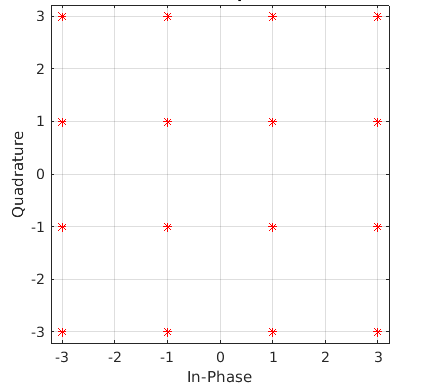
\includegraphics[width=0.85\textwidth]{resources/16QAM1.png}
		\label{fig:qam}
		\caption{Constellation of 16 QAM modulation scheme}
	\end{subfigure}%
	\begin{subfigure}{.5\textwidth}
		\setcounter{figure}{2}	
		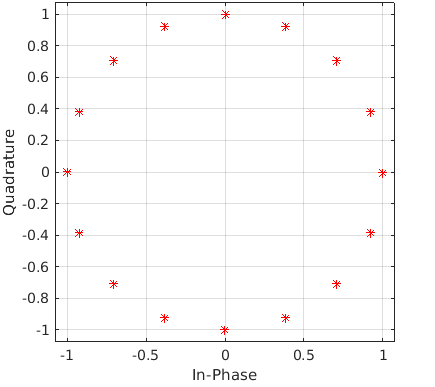
\includegraphics[width=0.85\textwidth]{resources/16psk2.png}
		\label{fig:mpsk}
		\caption{Constellation of 16 PSK modulation scheme}
	\end{subfigure}

	\caption{16-Ary Modulation sheme constellations}
	\label{fig:qampsk}
	
\end{figure}{}
From the figures \ref{fig:qampsk} it can be seen that 16-QAM has greater distances between constellations compared to 16-MPSK.
\\
\\
QAM exploits the fact that sine and cosine of the same frequency have a $90^{\circ}$  phase shift. This allows it to send two symbols using the same frequency doubling the symbol rate without doubling the bandwidth \cite{68}. It has also been proven in literature that QAM performs better than MPSK in Rayleigh Fading Channels \cite{67,65,66}. Due to arguments raised in sections \ref{sub:ask}--\ref{sub:psk} and in this section, QAM modulation is chosen as the suitable modulation scheme for this design.

\subsubsection{QAM Modulation and Demodulation}
\label{subsub:qam}
As previously mentioned, QAM modulates by impressing information on both the phase and amplitude. It exploits the fact that $cos(2\pi f_ct)$ and $sin(2\pi f_ct)$ are orthogonal. The modulated QAM signal takes the form:

\begin{equation}
 s(t) = A_I\sqrt{\frac{2}{T_s}}cos(2\pi f_ct) +  A_Q\sqrt{\frac{2}{T_s}}sin(2\pi f_ct) 
\end{equation}

\begin{center}
for $0 \le t \le T_s$
where $T_s$ is time in between symbols
\end{center}

$A_I$ and $A_Q$ are the information bearing discrete amplitude of the two quadrature carriers. Alternatively the symbol waveform can be expressed as:

\begin{equation}
s(t) = E\sqrt{\frac{2}{Ts}}cos(2\pi f_ct - \theta)
\end{equation}
Where $E =\sqrt{A_I^2 + A_Q^2} $ and $\theta = tan^{-1}(\frac{A_Q}{A_I})$ present the location of the symbol on the constellation, determined by the $log_2(M)$ bits to symbol mapper.
\\
\\
To demodulate, QAM demodulators use a coherent demodulator as illustrated by figure \ref{fig:demod}.

\begin{figure}[h!]
	\centering
	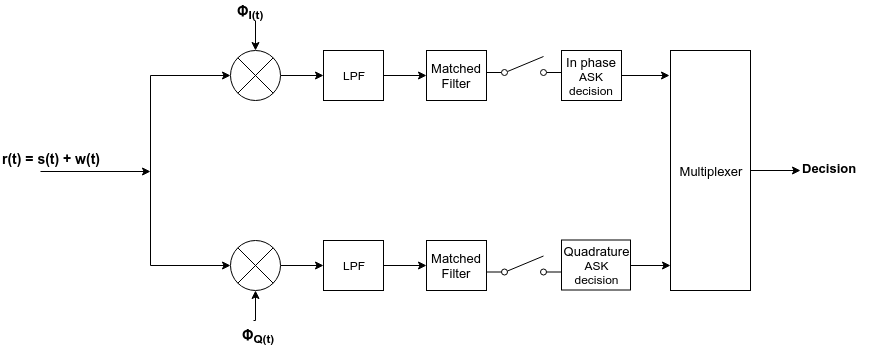
\includegraphics[width=\textwidth]{resources/demod.png}
	\caption{Coherent demodulator for QAM}
	\label{fig:demod}
\end{figure}
\vspace{12pt}
The distorted received symbol $r(t)$ is passed on to the demodulator as illustrated by figure \ref{fig:demod}. The symbol is then passed to the I and Q channels  where it is mixed with the local generated carriers $\phi_I(t) = \sqrt{\frac{2}{T_s}}cos(2\pi f_ct)$ and  $\phi_Q(t) = \sqrt{\frac{2}{T_s}}sin(2\pi f_ct)$. The mixed outputs are the passed to the Low Pass Filter (LPF) that rejects all high frequency components. The resulting signal is a basedband one, the baseband signal is then passed to the matched filter to improve the SNR \cite{B16}. The symbol demapper is then used to decode the received symbol and match it to the nearest corresponding symbol on the MQAM constellation by calculating the relative distance of the received symbol to all the symbols on the constellation. 
\\
\\
For this design 16-QAM is chosen. 16-QAM is chosen because it is just high enough to give a good spectral efficiency  whilst doing minimal damage on the BER \cite{B8}. The decision is also influenced by the desired spectral efficiency of the design. Spectral efficiency is given by equation \ref{eq:se}.

\begin{equation}
\label{eq:se}
S_E = \frac{1}{2}rlog_2(M)\alpha_M
\end{equation}
\begin{center}
	Where: $M$ is the modulation order, $\alpha_M$ is the MIMO coefficient and $r$ is given by equation \ref{eq:1}.
\end{center}

Using the above equation the $S_E$ with the subsystems implemented in section \ref{sec:encoding} and this section is $1.008\alpha_M$ bits/Hz. With an appropriate value of $\alpha_M$ the desired spectral efficiency can be met. The decision of 16-QAM is further supported in the results section.

\section{Channel Model}
\label{sec:channel}
As previously mentioned a channel adds noise, distorts and attenuates information bearing signals that propagate through it, leading to corruption of data. This design focuses on the two popular channel models, Additive White Gaussian Noise (AWGN) and Rayleigh Fading Channel (RFC). 

\subsection{AWGN}
\label{sub:awgn}
AWGN is common to every communication channel. It is a statistically random noise characterised by the effect of many random processes that occur in nature \cite{72}. The probability density function of AWGN follows a Gaussian distribution, as the name suggests. Given a sent signal $x(t)$, the received signal $r(t)$ that propagated through an AWGN channel is given by:

\begin{equation}
\label{eq:rawgn}
r(t) = x(t) + n(t)
\end{equation}

\begin{center}
Where $n(t)$ is AWGN noise with zero mean, $E\{n(t)\} = 0$.
\end{center}

The noise term $n(t)$ has power $N_0$, assuming that $x(t)$ has average power $E_b$ and the channel has bandwidth $W$, the $SNR$ of $r(t)$ is give by:

\begin{equation}
\label{eq:snr}
SNR = \frac{E_b}{N_0W}
\end{equation} 

Equation \ref{eq:snr} shows that AWGN affects the SNR which in turn affects the BER.

\subsection{Rayleigh Fading Channel}
\label{sub:rfc}
The RFC models the effect of propagation environment on an information bearing signal. The environment causes reflections and refraction leading to multipath and fading. The multipath then leads to intersymbol interference (ISI). In this design a RFC is modelled using the equation \ref{eq:rfc} below:

\begin{equation}
  \label{eq:rfc}
  h(t) = h_r(t) + jh_i(t)
\end{equation}

$h(t)$ is known as the channel coeffecient whilst $h_r(t)$ and $h_i(t)$ are the real and imaginary samples of a zero mean stationery Gaussian random process with variance $\sigma^2$ \cite{34}. The received signal $r(t)$ that passes through a RFC with AWGN is given by:

\begin{equation}
	\label{eq:rrfc}
	r(t) = h(t)x(t) + n(t)
\end{equation}

Where $ h(t) $ is given by equation \ref{eq:rfc}. Equation \ref{eq:rrfc} shows that the effects of of $ h(t) $ are multiplicative. The effect of h(t) is that it randomly rotates the phase and scales the amplitude of $r(t)$\cite{73}. The channel coherence time in this design is 1ms.

\section{MIMO}
\label{sec:mimo}
MIMO plays a great deal in mitigating the effects of fading and scattering presented in the previous section. As previously mentioned, MIMO exploits the attributes of a fading channel for diversity gain and high spectral efficiencies. This is achieved through its use of multiple transmit and receive antennas. What gives MIMO advantage over other schemes is its use of a third spatial dimension beyond frequency and time \cite{74}. Given a MIMO system with $N_t$ transmit antennas and $N_r$ receive antennas, the received signal vector $\vec{r}$ is given by :

\begin{equation}
\label{eq:mimo}
\vec{r} = \vec{H}\vec{x} + \vec{n}
\end{equation}

\begin{equation}
\label{eq:H}
\begin{bmatrix}
r_1 \\
r_2 \\
\vdots\\
r_{N_r}
\end{bmatrix}  = \begin{bmatrix}
h_{11} & h_{12} & \cdots & h_{1N_t} \\
h_{21} & h_{22} & \cdots & h_{2N_t} \\
\vdots &        &  \ddots      &  \vdots  \\
h_{N_r1}& h_{N_r2}&\cdots &h_{N_rN_t}
\end{bmatrix}
\begin{bmatrix}
x_1 \\
x_2 \\
\vdots\\
x_{N_t}
\end{bmatrix} + 
\begin{bmatrix}
n_1 \\
n_2 \\
\vdots\\
n_{N_t}
\end{bmatrix}  
\end{equation}

Where $ \vec{r} $ is a $ N_r\times1 $ column vector of received symbols, $ \vec{H} $ is a $ N_r\times N_t $ vector of channel coefficients, $ \vec{x} $ is a $N_t\times1 $ column vector of the transmitted signals and $\vec{n}$ is also a $ N_r\times1 $ column vector of AWGN noise. There exist two main types of MIMO, Space Time Block Codes (STBC) and Spatial Multiplexing.

\subsection{STBC}
\label{sub:stbc}
STBC is mostly used when there is no channel knowledge at the transmitter and it is mainly used for diversity gain. STBC achieves diversity gain by transmitting a number of replica of symbol streams through multiple antennas. This avails different version of the same received signal to get better reliability of the transmitted signal \cite{14}. A well known version of STBC is the Alamouti coding illustrated by figure \ref{fig:al}.

\begin{figure}[h!]
	\centering
	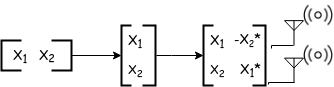
\includegraphics[scale=0.65]{resources/al.png}
	\caption{Flow diagram of Alamouti STBC}
	\label{fig:al}
\end{figure} 
From the figure it can be observed that the two input signals $(x_1, x_2)$ are multiplexed into two chains. The signals are then copied at different times to different antennas, to make what is called delayed diversity \cite{B8}. The two transmit antennas will then transmit the Alamouti encoded signals over two periods. First the original signals $(x_1,x_2)$ will be instantaneously transmitted followed by the copies in their second period \cite{14}. 

\subsection{Spatial Multiplexing}
\label{sub:sm}
Unlike STBC, Spatial Multiplexing is not intended to make transmission more robust, rather its prime focus is on increasing the spectral efficiency of a channel. To achieve this, Spatial Multiplexing divides data into streams, the streams are transmitted independently via separate antennas as illustrated by figure \ref{fig:sm}.

\begin{figure}[h!]
	\centering
	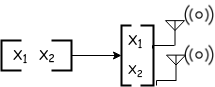
\includegraphics[scale=0.65]{resources/sm.png}
	\caption{Flow diagram of Alamouti STBC}
	\label{fig:sm}
\end{figure} 

The signals in figure \ref{fig:sm} are without any change in frequency band or transmission power. In the instance presented by figure \ref{fig:sm}, the spectral efficiency is doubled without any cost. Spatial Multiplexing can be used with or without Channel State Information (CSI).
\\
\\
Since the design focuses more on Spectral Efficiency and  since the CSI is known, Spatial Multiplexing is chosen as a suitable MIMO for the design. In this design a $4\times2$ Spatial Multiplexing MIMO is used. The reason for $4\times2$ is due to the fact that a higher number of antennas improves the BER. This in turn makes up for diversity in a sense.
\\
\\
Going back to equation \ref{eq:se}, $\alpha_M$ is given by:
\begin{equation}
\label{fig:nrnt}
\alpha_M = min(N_r,N_t)
\end{equation}
In the case of this design and taking all parameters in equation \ref{eq:se} into consideration, the $S_E = 2.00$ bits/Hz.

\subsection{MIMO Receivers}
\label{sub:rec}
The receive antennas of a MIMO system receive mixed multiple signals, that are rotated in phase and scaled in amplitude as previously mentioned in section \ref{sub:rfc}. A way of separating and reversing the channel coeffecients is through finding the inverse of the channel coeffecients matrix $\vec{H}$ \cite{37}. MIMO receivers have the ability to separate and equalise the received signal that is distorted by the RFC. There exist two popular MIMO receivers; The Zero Forcing (ZF) receiver and Minimum Mean Square Error (MMSE). Both of these receivers use what is called a pseudo-inverse to reverse the effect of the RFC channel.  

\subsubsection{The ZF Receiver}
\label{subsub:zf}
The ZF receiver applies the pseudo-inverse of the channel coeffecient matrix $\vec{W}$ to the received signal $\vec{r}$ to restore the transmitted signal $\vec{x}$. ZF brings the ISI to zero in a noise free case. It is most effective when the ISI is greater compared to the noise \cite{46}. The pseudo-inverse of the matrix $\vec{H}$  by ZF is given by:
\begin{equation}
\label{eq:zf}
\vec{W} = (\vec{H}^H\vec{H})^{-1}\vec{H}^H
\end{equation}

Despite its simple form, the ZF receiver amplifies noise, increasing the BER.

\subsubsection{The MMSE Receiver}
\label{subsub:mmse}
To minimise the ISI and additive noise, MMSE detects the transmitted signal through minimising the mean squared error \cite{B9}. The pseudo-inverse of the matrix $\vec{H}$ by MMSE is given by:

\begin{equation}
\label{eq:mmse}
\vec{W} = [\vec{H}^H\vec{H} + N_0\vec{I}]^{-1}\vec{H}^H
\end{equation}
\\
\\
MMSE generally performs better than ZF as it does not amplify noise \cite{46}. For this reason it is chosen as the receiver for this design. Therefore at the receiver the transmitted signal is recovered using equation \ref{eq:rec}:

\begin{equation}
	\label{eq:rec}
	\vec{\hat{x}} = \vec{W}\vec{r}
\end{equation}

\section{Simulation Results and Analysis}
\label{sec:results}
This section presents the results of the simulation of the system designed in sections \ref{sec:encoding}--\ref{sec:mimo}. All simulations are performed in MATLAB.

\subsection{BER for uncoded AWGN}
The first set of results come from section \ref{sec:encoding}. Figure \ref{fig:unc} below shows the effect of channel encoding in a AWGN channel.

\begin{figure}[h!]
	\centering
	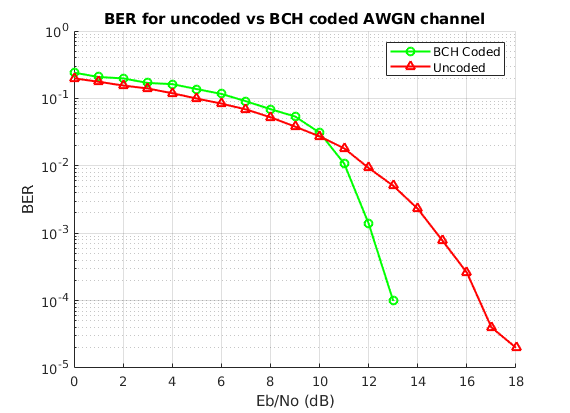
\includegraphics[scale=0.65]{resources/uncoded.png}
	\caption{Results of channel encoding vs no channel encoding in a AWGN channel}
    \label{fig:unc}
\end{figure}
\vspace{12pt}
The results of the figure clearly illustrates the need for channel encoding, as it can be seen that the BER curve of the coded scheme performs better. This is because encoding introduces parity to protect against and to correct errors in a channel, like the AWGN, as previously mentioned in section \ref{sec:encoding}.
\\
\subsection{BCH and QAM}
\label{sub:bchqam}
As already mentioned in the Introduction, the main requirement of this project is to design a codec that has a spectral efficiency of at least 2 bits/Hz. To meet the requirements 6 different combination of BCH and QAM which satisfy the requirements, assuming an $\alpha_M$ of 2, are simulated in AWGN channel to observe the one with an efficient BER. With $\alpha_M = 2$, $S_E$ from equation \ref{eq:se} becomes $S'_E$ given by:

\begin{equation}
\label{newse}
S'_E = rlog_2(M)
\end{equation}

The schemes together with their spectral efficiencies and other properties are shown in table \ref{t:schemes}.

\begin{table}[h!]
	\caption{BCH and QAM combinations that have $S_E  \ge 2$}
	\label{t:schemes}
	\begin{tabular}{|c|c|c|c|c|c|c|}
		\hline
		\textbf{\begin{tabular}[c]{@{}c@{}}Modu\\ lation\end{tabular}} & \multicolumn{3}{c|}{16-QAM} & \multicolumn{3}{c|}{64-QAM} \\ \hline
		\textbf{BCH} & BCH(31,16) & BCH(63,36) & BCH(127,64) & BCH(31,11) & BCH(63,24) & BCH(127,43) \\ \hline
		\textbf{t} & 3 & 6 & 10 & 5 & 7 & 14 \\ \hline
		\textbf{$S'_E$} & 2.06 & 2.29 & 2.02 & 2.13 & 2.29 & 2.03 \\ \hline
	\end{tabular}
\end{table}

All the schemes are simulated in MATLAB, figure \ref{fig:1664} illustrates the results. 

\setcounter{figure}{6} 
\begin{figure}
	\centering
	
	\begin{subfigure}{.5\textwidth}
		\centering
		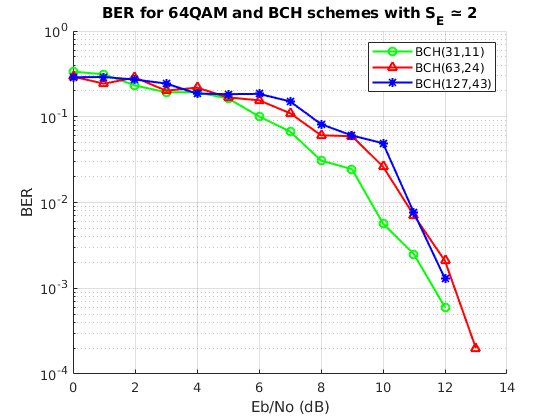
\includegraphics[width=\textwidth]{resources/bch64QAM.png}
		%\label{fig:64BCH}
		\caption{BER performance of 64-QAM with BCH}
	\end{subfigure}%
	\begin{subfigure}{.5\textwidth}	
		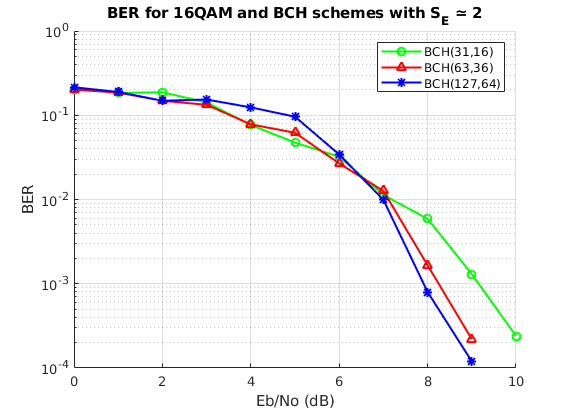
\includegraphics[width=\textwidth]{resources/bch16QAM.png}
		%\label{fig:16BCH}
		\caption{BER performance of 16-QAM with BCH}
	\end{subfigure}
	
	\caption{BCH and QAM combinations that have $S_E  \ge 2$}
	\label{fig:1664}
	
\end{figure}{}
\vspace{12pt}
From figure \ref{fig:1664} it can be seen that the combinations with 16-QAM perform better than those with 64-QAM even though 64-QAM combinations have higher error correcting BCH as per table \ref{t:schemes}. This goes to show that modulation plays a great role in BER compared to encoding. The 16-QAM constellations have a greater distance between them compared to those of 64-QAM, this implies that less demodulation errors are made in 16-QAM compared to 64-QAM even though it has BCH schemes that have greater error correcting capabilities.
\\
\\
Within 16-QAM BCH(127,64) performed better than all the BCH schemes. This is because BCH(127,64) has higher error correcting capabilities compared to all the BCH schemes in 16-QAM as per table \ref{t:schemes}. All these results influenced the decisions made in section \ref{sec:encoding} and section \ref{sec:modem} for the type of BCH and the modulation order respectively.

\subsection{MIMO and Antenna Configuration}
This subsection presents the results for MIMO in Rayleigh Fading Channel. For MIMO and RFC two antenna configurations are simulated with the chosen channel encoding of BCH(127,64) and modulation of 16-QAM. The two antenna configurations are $2\times2$ and $4\times2$. To reverse the effect of the channel coeffecient $\vec{H}$, MMSE is used as discussed in the earlier section. Figure \ref{fig:anten} below illustrates the results for the different configurations.

\begin{figure}[h!]
	\centering
	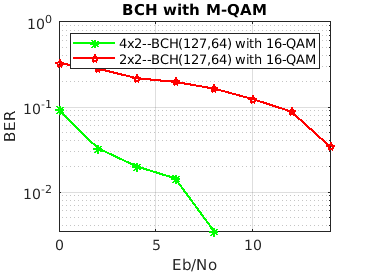
\includegraphics[scale=1]{resources/twotwoV2.png}
	\caption{BER for different antenna configurations in RFC}
	\label{fig:anten}
\end{figure}
From  figure \ref{fig:anten} it can be seen that a MIMO system with four receive antennas performs better than one with two receive antennas. This is because more antennas increase diversity and in turn improves the BER. This explains the decision made in section \ref{sub:sm}.
\\
\\
The final MIMO codec system designed for a Rayleigh Fading Channel is a $4\times 2$ MMSE receiver 16-QAM BCH(127,64) codec. The codec has spectral efficiency of 2.00 bits/Hz as per equation \ref{eq:se}. The final codec, compared with AWGN, is illustrated by figure \ref{fig:final}.

\begin{figure}[h!]
	\centering
	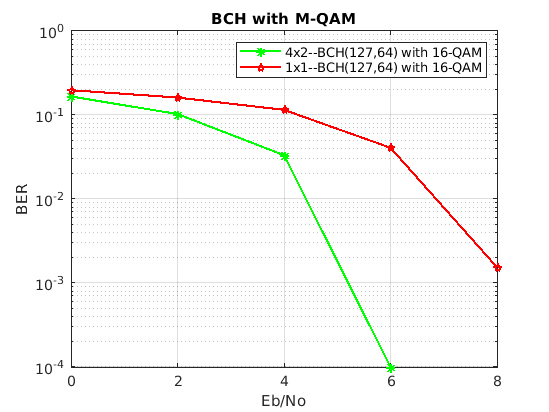
\includegraphics[scale=1]{resources/fourtwoV1.png}
	\caption{BER for RFC performance of the final codec with $S_E$ = 2.00 bits/Hz vs BER in AWGN for no RFC and MIMO}
	\label{fig:final}
\end{figure}

From figure \ref{fig:final} it can be seen that the codec performs better than the pure AWGN coded channel.

\section{Future Recommendations}
In future the system could use Convolutional codes concatenated with RS codes for FEC. In this configuration, Convolutional codes do most of the work, whilst Reed Solomon cleans whatever is left behind. Exploration into using the Maximum Likelyhood (ML) receiver could also be taken into consideration. Literature has proven ML to perform better than MMSE and ZF in retrieving transmitted signals.

\section{Environmental, Social and Economic Impacts} 
The proposed solution promises to use less power and therefore will have a lower carbon footprint on the environment. Because of increased signal range less basestations will need to be setup, saving power used per basestation and further reducing the carbon footprint.
\\
\\
MIMO also promises more robust privacy compared to other system. Since the information is carried in multiple waves hackers will not know which to attack, making it less prone to hacking. 
\\
\\
Since data is expensive, MIMO promises cheaper infrastructure. This may lead to cheaper data bundle prices, making the internet available to the less privileged. This will also stimulate a spirit of entrepreneurship in online markets and also stimulate growth of small enterprises onto the online market. All this leads to an increased GDP.

\section{Conclusion}
This paper presented the design of a robust codec for fading channel. The codec use BCH(127,64) for channel encoding, 16-QAM for modulation and a $4\times2$ Spatial Multiplexing MIMO antenna configuration. At the receiver of the MIMO architecture a MMSE receiver is used to equalise and sum the received distorted signals. The results show that modulation schemes greatly affect BER performance, they also show that more antennas improve diversity. Overall the codec achieved a spectral efficiency of 2.00 bits/Hz which meets the design requirements.  
%% References
\bibliographystyle{IEEEtrans}
\bibliography{references}
\newpage
\begin{appendices}
	
	\section*{Appendix A}
	
	\subsection*{Brief Overview}
	A codec is a device or computer program that encodes or decodes a digital data stream or signal. The function of a codec is to make communication networks more faster and efficient. A codec seeks to make communication between devices faster and less prone to errors. A Rayleigh fading channel on the other hand is a representation of the journey information takes especially in urban areas. The information signals are reflected and refracted by buildings causing them to loose energy and fade. Normal codecs struggle in Rayleigh Fading channels due to its nature, they lead to poor performances, poor download speeds,  poor reliability, more dropped calls, failed downloads and lagging stream. The solution to all these problems is Multiple Input Multiple Output (MIMO). MIMO takes advantage of the reflection and refraction of information signals by using multiple antennas to send and receive information. By using multiple antennas MIMO allows more users to connect to a specific network. A MIMO communication system is also faster compared to a normal one. Some wifi and 4G networks are already using MIMO to make communication easier and swifter.
	
	
	\subsubsection*{Social Impacts}
	Communication networks have since allowed humans to have better interaction, bringing people together even though they are thousands of miles apart. MIMO allows more people to connect to a network, this means people can communicate and connect effectively with less dropped calls and less latency in video calls or video streams. Higher download speads also mean people can get faster access to information. Hacking and information privacy are issues of the modern age. MIMO minimizes the chances of one being hacked due to its multiple transmit antennas to send information.
	
	\subsubsection*{Economic Impacts}
	A lot of developing countries do not have proper network infrastructure, this is mainly due costs \cite{acm}. MIMO is cost effective to implement compared to other communication channels. Due to its increase in range, fewer base stations could be built saving governments and businesses money \cite{50}. With the increased rand and speeds, more learners could also connect , to learn and research effectively improving the pass rate and boosting the economy. More entrepreneurs such as web developers, youtube bloggers and Instagram influencers will emerge. 
	
	
	\subsubsection*{Environmental Impacts}
	Due to to an increased ranges as mentioned earlier, there will be less base stations per area meaning less power consumption from base stations by MIMO base stations. MIMO networks also use less radio-transmission power so there is less battery drainage on portable devices such as cellphone \cite{50}. All this means MIMO will have lesser carbon foot print compared to other systems. However, the implementation of MIMO may cause e-waste as some of the old infrastructure might have to be removed. On the long term, MIMO will have a positive environment compared to other systems.
	
	\end{appendices}


\end{document}          
